\documentclass[letterpaper,twocolumn,openany,nodeprecatedcode]{dndbook}
\usepackage[english]{babel}
\usepackage[utf8]{inputenc}
\usepackage[singlelinecheck=false]{caption}
\usepackage{lipsum}
\usepackage{listings}
\usepackage{shortvrb}
\usepackage{eso-pic}
\usepackage{tikzpagenodes}
\usepackage{multicol}
\usepackage{float}
\usepackage{graphicx}

\captionsetup[table]{labelformat=empty,font={sf,sc,bf,},skip=0pt}

\MakeShortVerb{|}

\lstset{%
  basicstyle=\ttfamily,
  language=[LaTeX]{TeX},
  breaklines=true,
}
%Colocar imagem no fundo
\newcommand{\Background}{%
  \begin{tikzpicture}[remember picture,overlay]
    \node at (current page.center) {
      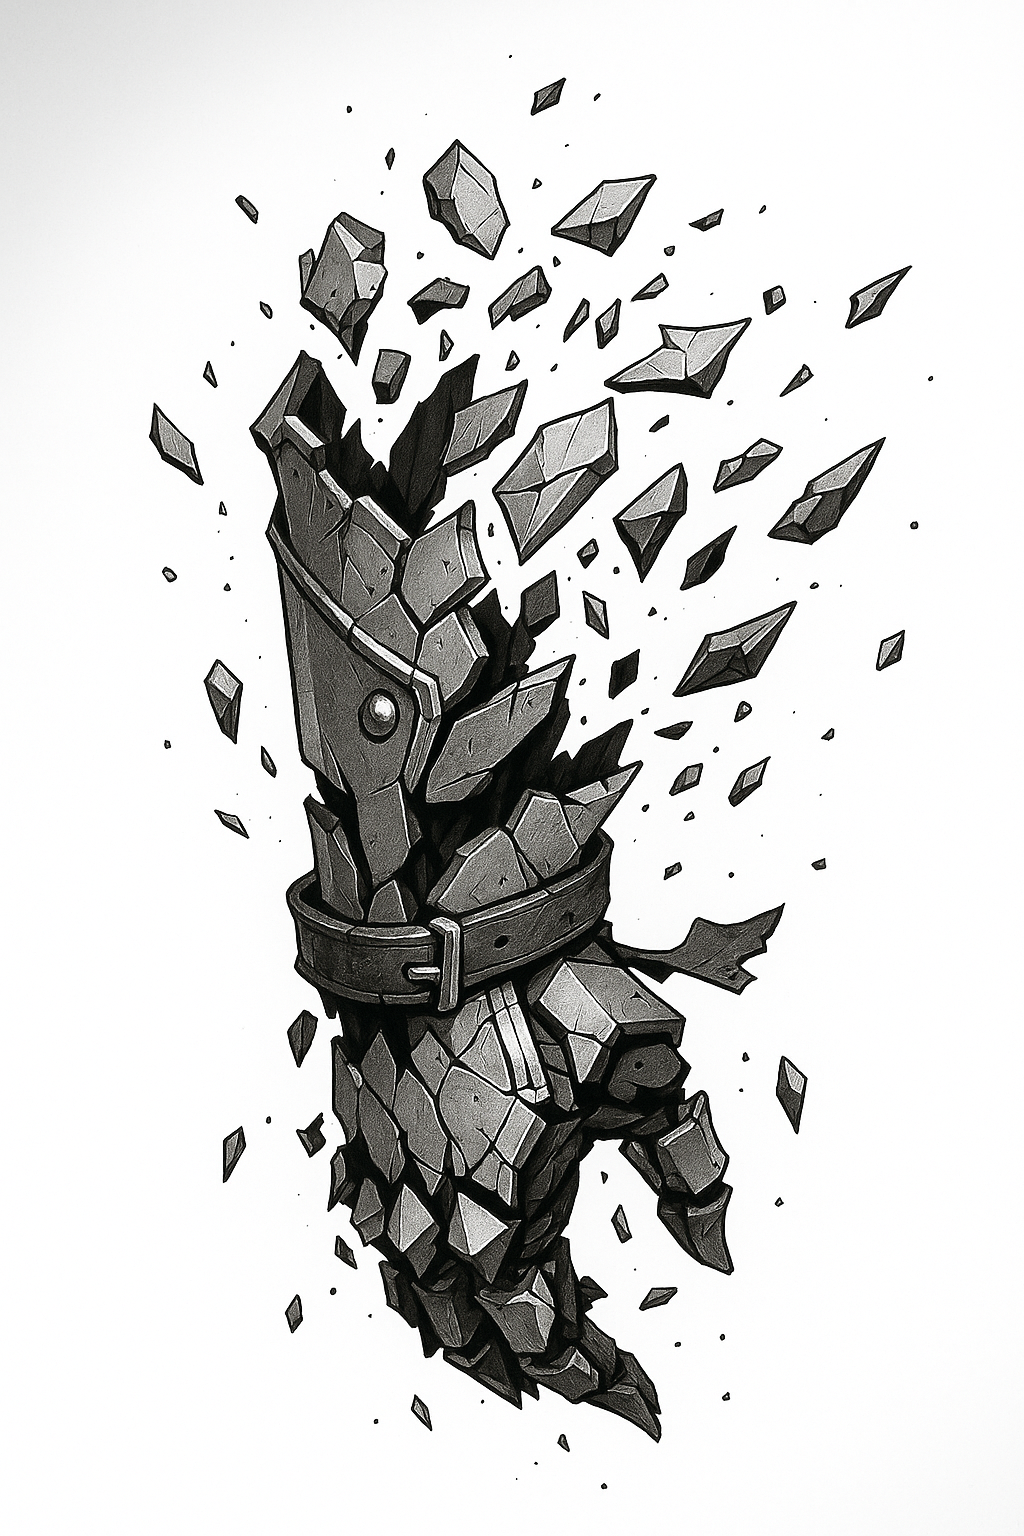
\includegraphics[width=\paperwidth,height=\paperheight]{img/Manopla estilhaçada de Rakaar.png}};
  \end{tikzpicture}
}

\begin{document}

\frontmatter
\begin{titlepage}
    \Background
\end{titlepage}
\section{Manoplas e Semelhantes}

\begin{tcolorbox}[
  enhanced,
  colback=white,
  colframe=black!85,
  boxrule=0.9pt,
  arc=2mm,
  drop shadow,
  left=6pt,
  right=6pt,
  top=6pt,
  bottom=6pt,
  width=\textwidth
]
\begin{DndTable}[header= Novas Armas]{XcXcXc}
    \textbf{Arma} & \textbf{Custo} & \textbf{Dano} & \textbf{Peso} & \textbf{Propriedades} & \textbf{Maestria} \\
    Armas Simples &  &  &  &  &  \\
    \hspace{0.5cm}Soco Inglês & 5 po & 1d4 concussão & 0,2 kg & Acuidade, leve, punho & Ágil \\
    \hspace{0.5cm}Cesto & 5 po & 1d4 concussão & 1 kg & Acuidade, leve, punho & Lentidão \\
    \hspace{0.5cm}Cesto com espinhos & 10 po & 1d6 concussão & 2 kg & Leve, punho & Drenar \\
    Armas Marciais &  &  &  &  &  \\
    \hspace{0.5cm}Manopla de combate & 30 po & 1d8 concussão & 2,5 kg & Punho, reforçado & Empurrar \\
    \hspace{0.5cm}Manopla de força & 85 po & 1d10 concussão & 7,5 kg & Desajeitado, massivo, pesado, punho, reforçado & Garantido \\
\end{DndTable}
\end{tcolorbox}

\subsection{Propriedades das Armas}
Alguams das armas acima tem propriedades que não são encontradas no livro do jogador.
Estas propriedades são descritas a seguir:
\vspace{\baselineskip}

\paragraph{Desajeitado} Esta arma torna difícil segurar objetos frágeis e realizar movimentos ágeis.
Você possui disvantagem em testes de Destreza (Prestidigitação) enquanto estiver vestindo esta arma.
Se você estiver vestindo duas armas com essa propriedade, uma em cada mão, o dano de cada uma aumenta em um dado.
\vspace{\baselineskip}

\paragraph{Massivo} Seu atributo Força deve ser 16 ou maior para empunhar esta arma eficientemente.
Caso contrário, você possui desvantagem em toda ação que envolver o braço que segura esta arma.
\vspace{\baselineskip}

\paragraph{Punho} Esta arma envolve sua mão e exige que ela esteja vazia para ser usada eficientemente, mas pode ser usada
para segurar outros objetos ou armas. Além disso, esta arma não pode ser desarmada de você.
\vspace{\baselineskip}

\paragraph{Revestido} Esta arma é coberta ou feita com placas de metal, garantindo um bonus de +1 a sua CA quando vestida.
Este bonus não é aplicado quando você veste uma armadura pesada.
\end{document}